\chapter{Introduction}
\label{chp:b1}

Autonomous cars received a great deal of attention over the last two decades
and started to be a reality in the last few years with several level of
autonomy from driving assistance level to full autonomy
\cite{Holstein2018EthicalAS}. In quest of fully autonomous vehicles, a number
of competitions were organized to stimulate researchers' interest
\cite{Buehler2007The2D, Buehler2009TheDU}. These events started with autonomous
cars driving on desert roads with only static obstacles and evolved to a point
where the cars survived a simple form of everyday traffic including highway
driving, overtaking, intersections, and parking. These challenges led to
state-of-art software architectures which decompose the driving problem into
components such as perception, planner, and controller. Each of these
components was also powered by state-of-art algorithms that shaped the today's
autonomous vehicles.

Meanwhile, the progress in deep learning techniques along with the increase of
storage and computational power in the computer market made a breakthrough in
computer vision. These advances not only boosted the decomposition-based
approach in perception side, but also revived the existing idea of learning a
mapping from raw camera images to steering commands \cite{Bojarski2016EndTE},
which is followed by the idea of learning driving affordance indicators such as
distance to the center of the ego lane, orientation of the car relative to the
road, and distance to the other cars from the images so that steering and speed
commands can be computed with a dedicated controller based on these affordances
\cite{Chen2015DeepDrivingLA}.

Being an elegant and promising solution, learning affordances from the raw
images requires additional tooling for data acqusition in order to compute and
record affordance indicators per image. The choice of affordances for a smooth
driving experience also presents its own challenge.

Learning a direct mapping to the steering commands quickly reaches its limit
when the driving scenario becomes more complicated than tracking a curvy
road. Introduction of traffic regulations, overtaking, and lane keeping
policies remains too abstract to be captured in such a mapping. Furthermore,
human drivers tend to take different actions at different times even for the
same scenarios. Different actions on the similar raw images in the training set
easily confuses the model \cite{Chen2015DeepDrivingLA}. Last but not least,
end-to-end nature of this approach presents difficulties in understanding and
debugging the behavior of the vehicle.

Existing decomposition-based approaches heavily depend on a high-definition map
of the driving environment, which often loses its validity due the changing
streets or constructions on the roads. Autonomous driving in urban scenarios
without an accurate map has been studied extending an existing traffic scene
segmentation dataset with ego lane, parallel lane, and opposite lane
annotations \cite{Meyer2018DeepSL}, but it is yet to be deployed and tested on
a car. For novel methods like this instance, a low-cost and risk-free solution
could be the use of a small-scale car for initial on-road testing.

Present smale-scale driverless car studies either focus on directly learning
steering commands from the images \cite{Bechtel2017DeepPicarAL,
Do2018RealTimeSC} or implement a decomposed architecture using traditional
computer vision techniques to detect ego lane lines and few traffic signs
\cite{Blaga2018MiniatureAV}. Despite the existence of powerful small-scale
autonomous car platforms in the hardware side \cite{Karaman2017ProjectbasedCA},
related studies in the software side fail to keep up with the advances in
self-driving car technologies. One possible reason behind this lag could be the
lack of datasets for mini cars.


\section{Problem Definition}

We seek autonomous driving solutions to a number of traffic scenarios specified
by a mini autonomous car competition, OpenZeka MARC 2019 \cite{OpenZekaMARC}.
Our requirements are mostly derived from the competition rules as follows:

\begin{itemize}
  \item The mini car shall follow lane at 0.6 m/s average speed in a two-lane
    road given in Figure \ref{figure:openzeka-race-course}.
  \item The mini car shall slow down to 0.5 m/s average speed on traffic signs
    and signals given in Figure \ref{figure:openzeka-traffic-signs}.
  \item The mini car shall overtake a waiting car on the right lane and steer
    back to the right lane.
  \item The mini car shall reactively avoid obstacles.
  \item The car shall climb up and climb down the bridge given in Figure
    \ref{figure:openzeka-race-course}.
  \item The mini car shall choose to go straight straight when it encounters
    Straight or Right Turn sign given in.
  \item The mini car shall stop on red light and move on green light.
  \item The mini car shall change left when it is close to a construction zone
    on the right lane as indicated by Keep Left sign.
  \item The mini car shall pass the loose road section indicated by a Loose
    Road sign.
  \item The mini car shall wait for pedestrians on crosswalks indicated by a
    Crosswalk sign.
  \item The mini car shall turn right after Parking sign into the parking lot
    given in Figure \ref{figure:openzeka-race-course}.
  \item The mini car shall stop on any of the free parking slots.
\end{itemize}

\begin{figure}[h]
  \centering
  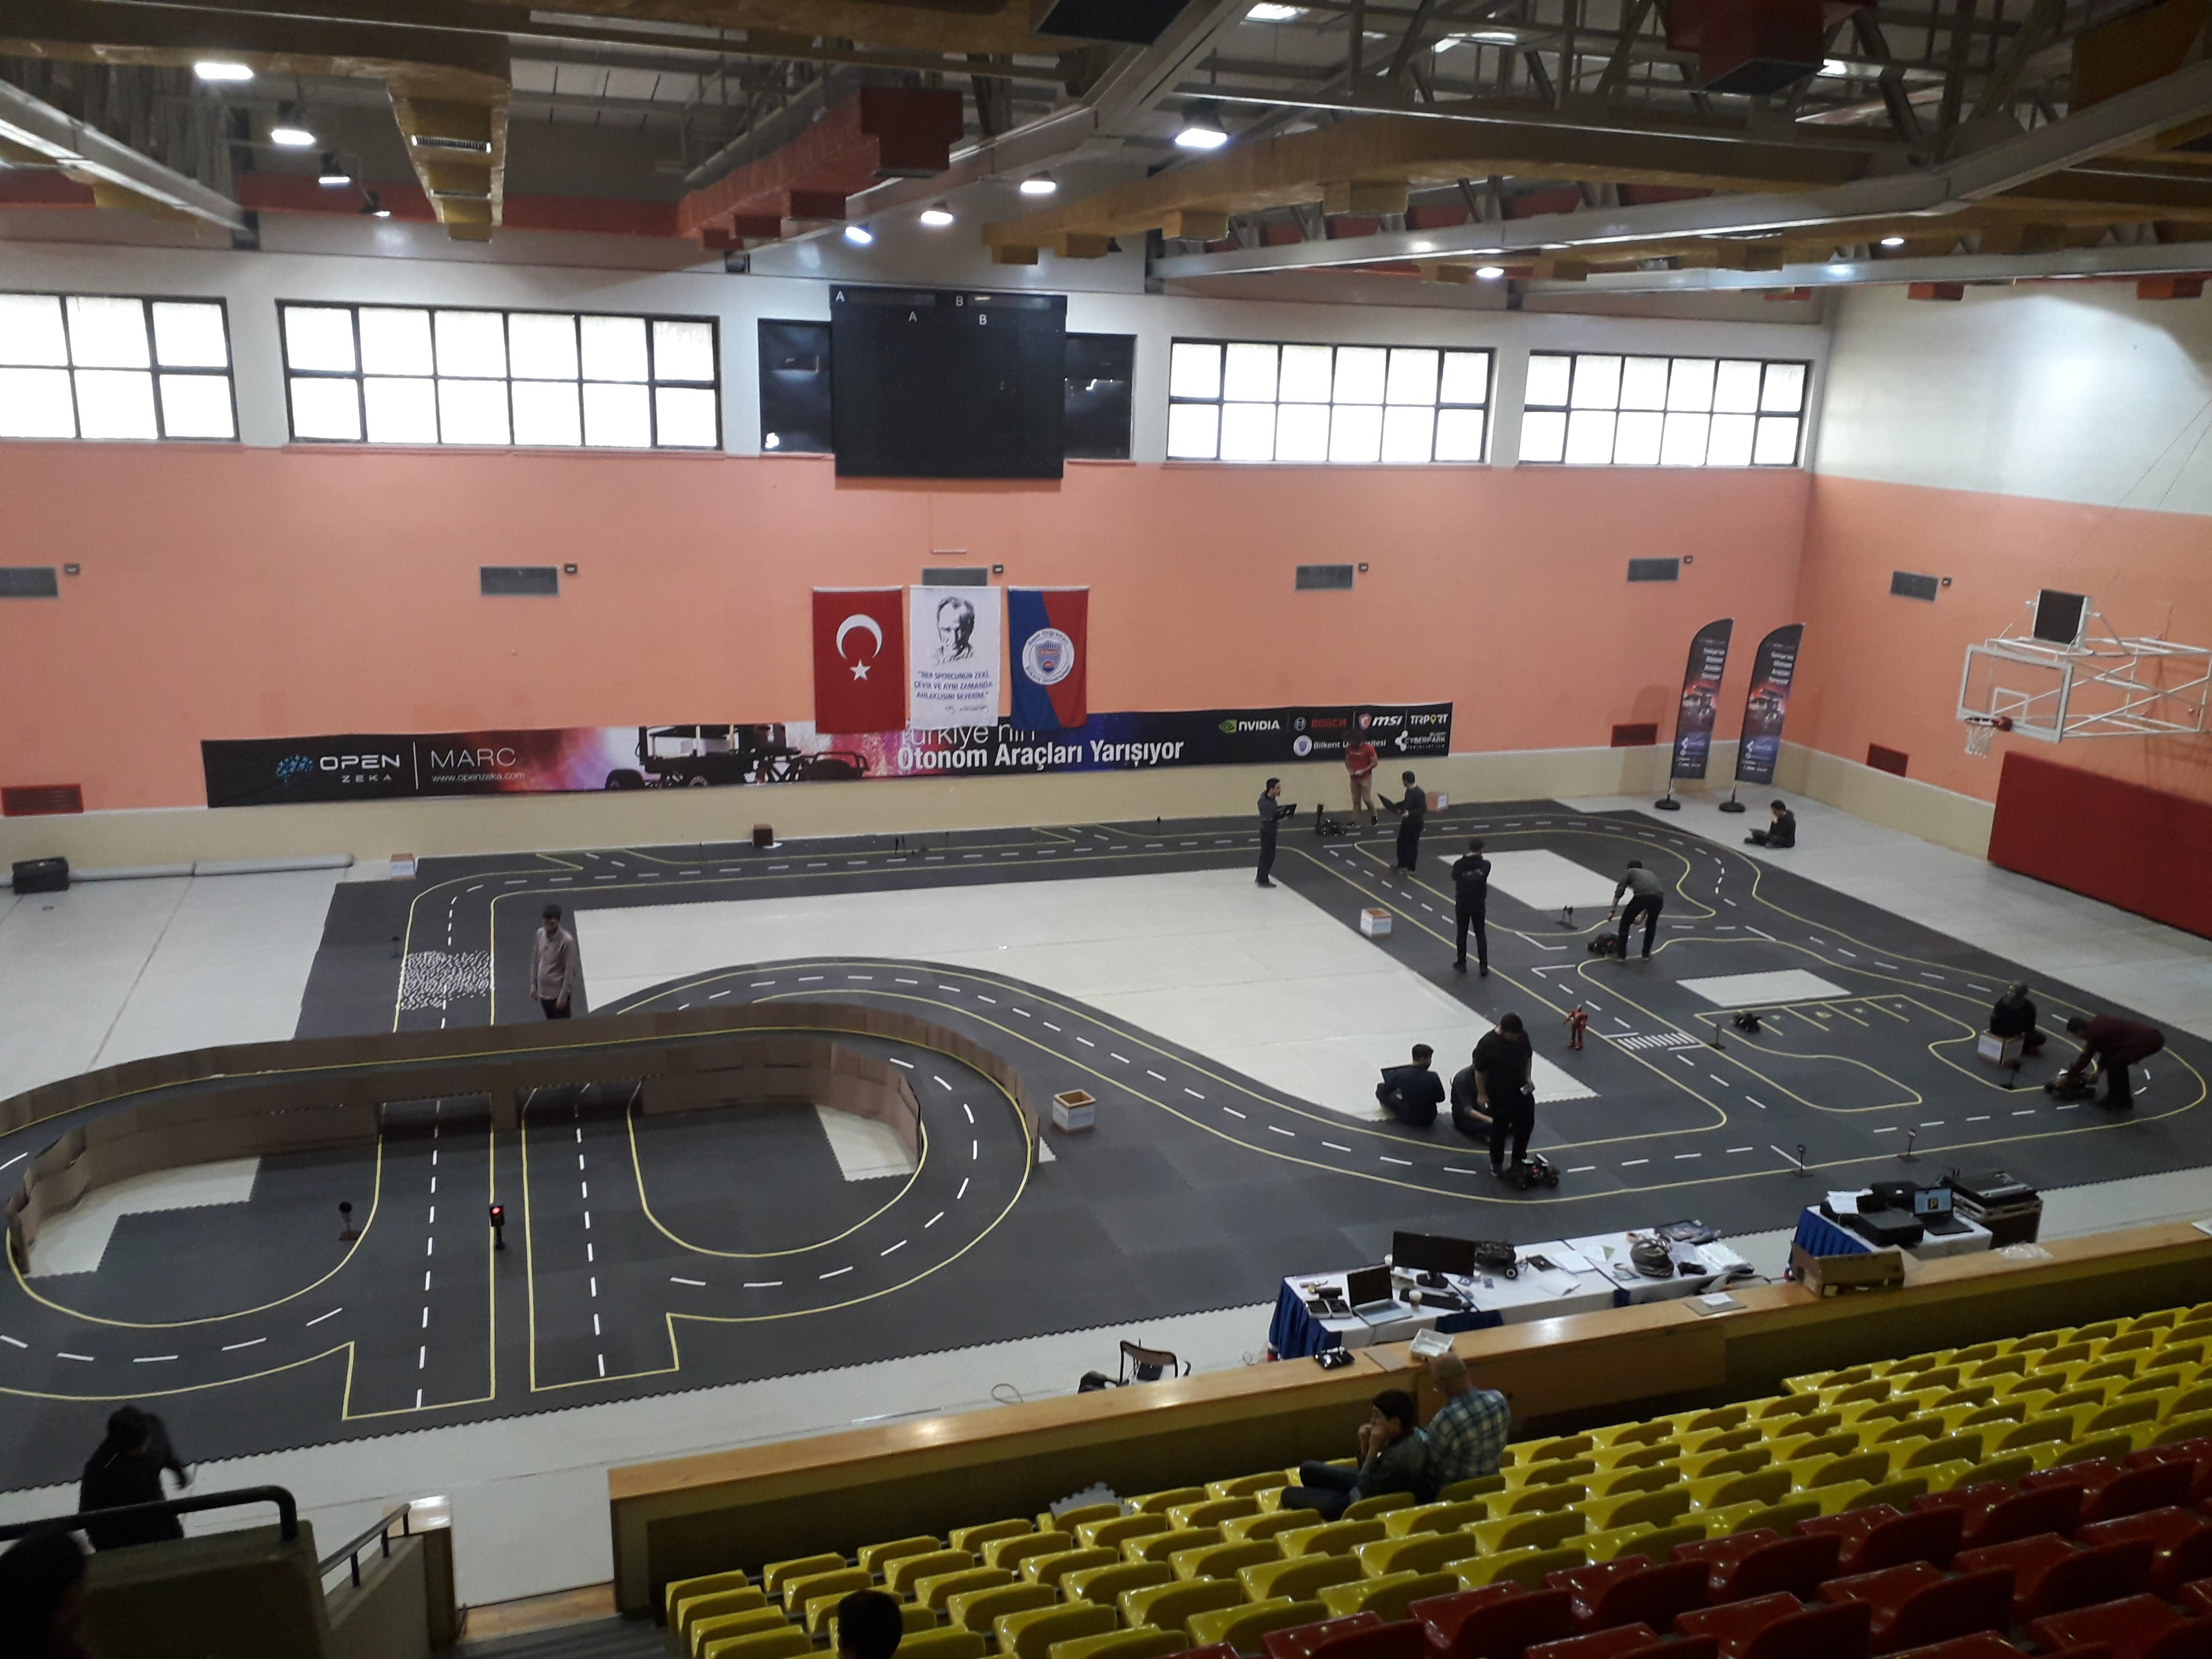
\includegraphics[width=.8\textwidth]{figures/openzeka-race-course.jpeg}
  \caption{OpenZeka 2019 MARC race course.}
  \label{figure:openzeka-race-course}
\end{figure}

\begin{figure}[h]
  \centering
  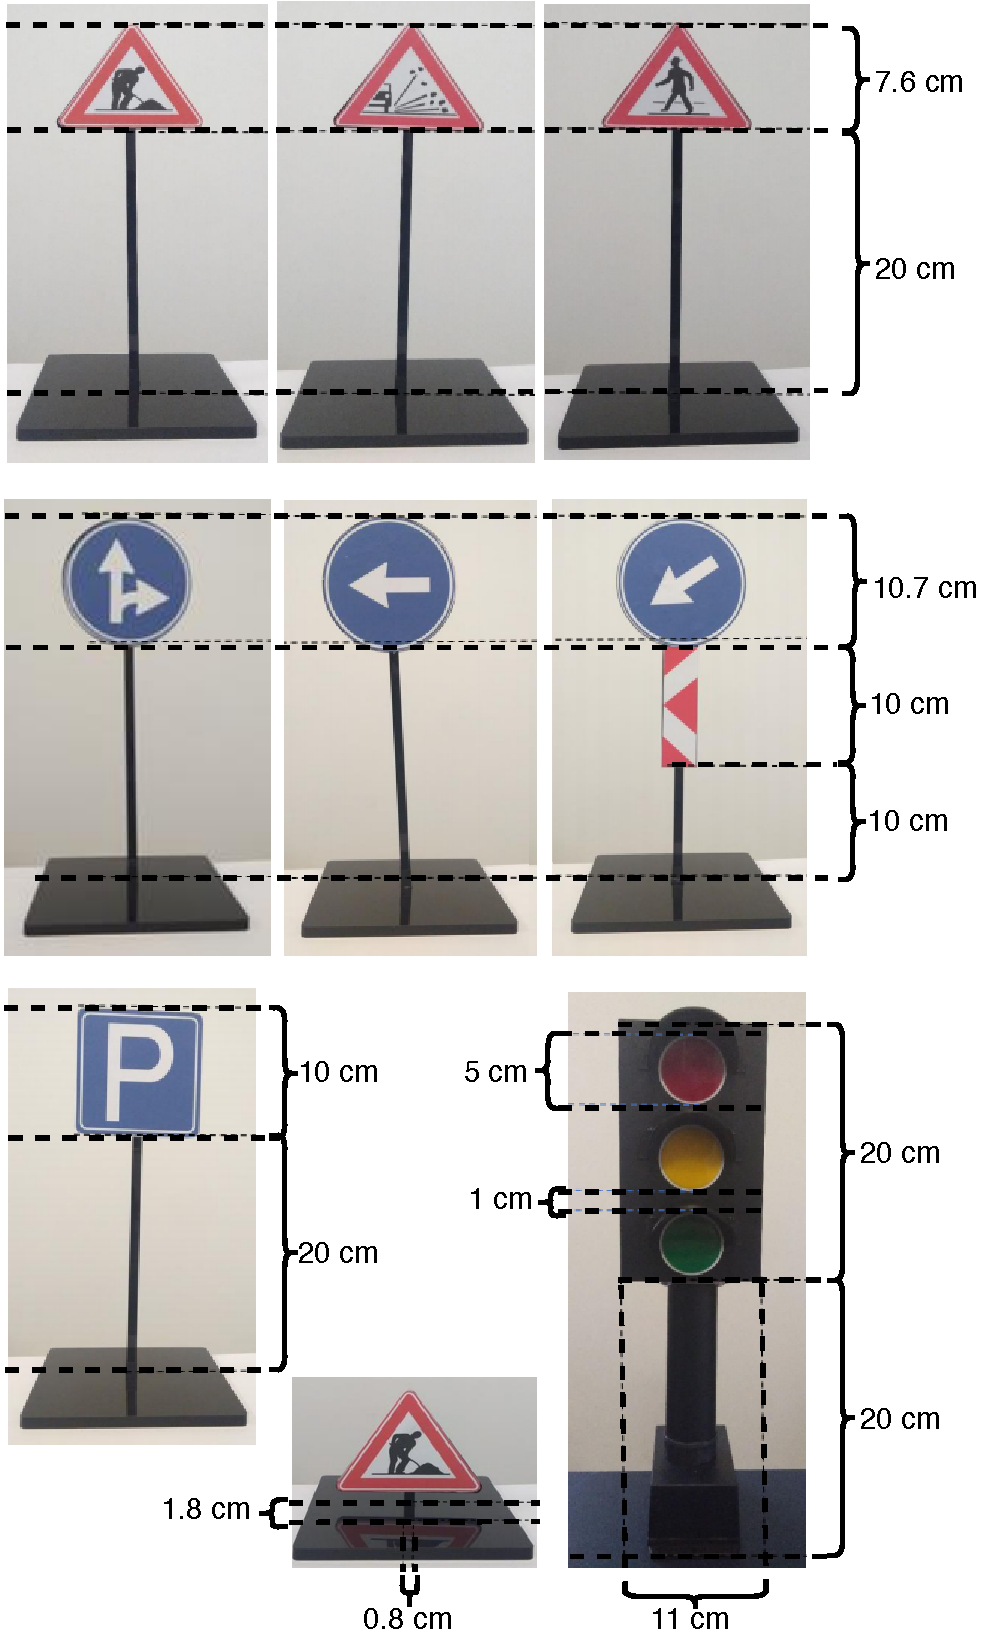
\includegraphics[width=.8\textwidth]{figures/openzeka-traffic-signs.pdf}
  \caption{Traffic signs and light specifically design for mini cars by
  OpenZeka.}
  \label{figure:openzeka-traffic-signs}
\end{figure}

\section{Contributions}

The main contribution of our study is as follows:

\begin{itemize}
  \item \textbf{Pixel classification dataset for mini cars:} Existing traffic
    scene datasets exclusively for real-scale cars \cite{Huang2018TheAD,
    Cordts2016TheCD, Geiger2012AreWR, Neuhold2017TheMV}. This poses a
    difficulty for on-road testing of the novel methods on mini-cars. We
    present a dataset with pixel-level annotations for mini cars.
  \item \textbf{Extended traffic sign and signal classification dataset:} We
    merge existing traffic sign classification datasets
    \cite{Timofte2009MultiviewTS, Stallkamp2012ManVC, Shakhuro2016RussianTS,
    Serna2018ClassificationOT, MaldonadoBascn2007RoadSignDA} for our scenarios
    and semi-automatically extend the dataset by cropping the segmented sign
    regions from our left camera images.
  \item \textbf{Development of a lane detector:} We build our lane detector on
    the approach proposed in \cite{Meyer2018DeepSL}. This approach essentially
    segments the road into ego lane, parallel lane, and opposite lane. It then
    extracts a center line for the ego lane. For our scenarios, we skip the
    opposite lane and further segment the parallel lane into right and left
    lanes.  Unlike \cite{Meyer2018DeepSL}, we are interested in finding center
    line curves for ego lane and also the neighboring parallel lanes. Our
    apprach saves us from analyzing the parallel lane pixels for right and left
    categorization for the curve estimation.
  \item \textbf{Local optimal trajectory planner for structured environments:}
    It is common that state-of-art autonomous vehicles relies on detailed maps
    to provide a reference line to the local planner for structural
    environments (i.e., environments with explicit drivable corridors), often
    by means of a global planner \cite{Thrun2006StanleyTR,
    Montemerlo2009JuniorTS, Kato2018AutowareOB}. We implemented a Frenet
    optimal trajectory planner \cite{Werling2010OptimalTG} without a map using
    exclusively the online computed lane centers as a source of the reference
    line.
  \item \textbf{Decomposed architecture for autonomous driving:} Autonomous
    vehicle architectures span wide range of computer science research areas
    including but not limited to computer vision, path planning, automata
    theory, control theory, and distributed systems.  Each of these areas comes
    with many problems and various alternative solutions to those problems. We
    put together a decomposed architecture with a selected set of solutions
    from different domains.
\end{itemize}

\section{Organization}

The organization of this thesis as follows. Chapter 2 discusses various
autonomous driving approaches and algorithms often used in search of autonomy
hightlighting their advantages and disadvantages.

Chapter 3 presents our hardware configuration and software architecture at a
high level. In Chapter 3, we also introduce our simulation environment that
accelerated the development and verification processes while implementing the
software components.

Chapter 4 provides a detailed description of our scene interpretation module in
which we implement perception and behavior planning capabilities of the car.
First, We present our segmentation model which is used to parse the current
scene into lanes and traffic signs. Second, we introduce our lane center line
extraction method based the parsed lane semantics. Third, we discuss our
traffic sign classification approach over the sign locations proposed by
segmentation model. Fourth, we review our obstacle detection method. Finally,
we explain our behavioral layer that implements a hierarchical finite state
machine that regulates the decisions made by the car based on the perception
capabilities.

Chapter 5 is dedicated to our trajectory planner and control algorithms. We
start with introducing Frenet frame on a lane segment and then we explain how
we plan an optimal trajectory based on the lane center lines provided by scene
interpretation module. In the second half of this chapter, we derive pure
pursuit algorithm that computes steering commands to execute our optimal
trajectories.

Chapter 6 presents our datasets, experiments, and results. In Chapter 6, we
evaluate our segmentation and classification models. Then, we demonstrate the
actions our car takes in response to various traffic scenarios.

Chapter 7 concludes our arguments by summarizing our approach to autonomous
driving with its limitations and suggesting directions for future work.
